\documentclass[dvipdfmx]{ujarticle}
\usepackage{eee}

\begin{document}
\title{平成30年 電磁気学II 第1回小テスト}
\date{}
\author{大山主朗}

\maketitle

\section{以下の(a)及び(c)に示す物理定数は電磁気学を修めた者であれば常識的に覚えていなければならない数値である.それぞれの値を示せ.}
\begin{enumerate}[(a)]
	\item 真空の誘電率$\varepsilon_{0}:8.854 \times 10^{-12}\,\rm{F/m}$
	\item 真空の透磁率$\mu_{0}:1.257 \times 10^{-6}\,\rm{H/m}$
	\item 電子の電荷$e:-1.602 \times 10^{-19}\,\rm{C}$
\end{enumerate}

\section{一辺の長さ$a$の正方形がある.点Aに$-2q[\rm{C}]$,点Bに$+1q[\rm{C}]$,点Cに$−4q[\rm{C}]$,点Dに$+3q[\rm{C}]$,が点Oに$-q[\rm{C}]$の点電荷が存在するとき,点Oにある電荷にはたらく力$F$の大きさを求めよ.ただし,$q>0$とする.}
\begin{align*}
		\boldsymbol{F}_{A}&=\frac{1}{4\pi \varepsilon_{0}}\frac{-2q(-q)}{\left(\left(-\frac{a}{2}\right)^{2}+\left(\frac{a}{2}\right)^{2}\right)^{3/2}} \left\{-\frac{a}{2}\boldsymbol{i}+\frac{a}{2}\boldsymbol{j}\right\}\,[\rm{N}]\\
		\boldsymbol{F}_{B}&=\frac{1}{4\pi \varepsilon_{0}}\frac{q(-q)}{\left(\left(-\frac{a}{2}\right)^{2}+\left(-\frac{a}{2}\right)^{2}\right)^{3/2}} \left\{-\frac{a}{2}\boldsymbol{i}-\frac{a}{2}\boldsymbol{j}\right\}\,[\rm{N}]\\
		\boldsymbol{F}_{C}&=\frac{1}{4\pi \varepsilon_{0}}\frac{-4q(-q)}{\left(\left(\frac{a}{2}\right)^{2}+\left(-\frac{a}{2}\right)^{2}\right)^{3/2}} \left\{\frac{a}{2}\boldsymbol{i}-\frac{a}{2}\boldsymbol{j}\right\}\,[\rm{N}]\\
		\boldsymbol{F}_{D}&=\frac{1}{4\pi \varepsilon_{0}}\frac{3q(-q)}{\left(\left(\frac{a}{2}\right)^{2}+\left(\frac{a}{2}\right)^{2}\right)^{3/2}} \left\{\frac{a}{2}\boldsymbol{i}+\frac{a}{2}\boldsymbol{j}\right\}\,[\rm{N}]\\
		\boldsymbol{F}&=\boldsymbol{F}_{A}+\boldsymbol{F}_{B}+\boldsymbol{F}_{C}+\boldsymbol{F}_{D}\\
		&=\frac{1}{4\pi \varepsilon_{0}}\frac{q^{2}}{\left(\left(\frac{a}{2}\right)^{2}+\left(\frac{a}{2}\right)^{2}\right)^{3/2}}\left\{\left(-a+\frac{a}{2}+2a-\frac{3}{2}a\right)\boldsymbol{i}+\left(a+\frac{a}{2}-2a-\frac{3}{2}a\right)\boldsymbol{j}\right\}\\
		&=\frac{1}{4\pi \varepsilon_{0}}\frac{q^{2}}{\left(\frac{a^{2}}{4}\right)^{3/2}}\left(-2a\boldsymbol{j}\right)\\
		&=\frac{1}{4\pi \varepsilon_{0}}\frac{8q^{2}}{a^{3}}\left(-2a\boldsymbol{j}\right)\\
		&=-\frac{4q^{2}}{\pi \varepsilon_{0}a^{2}}\,\boldsymbol{j}\,[\rm{N}]\\
		|\boldsymbol{F}|&=\frac{4q^{2}}{\pi \varepsilon_{0}a^{2}}\,[\rm{N}]
\end{align*}

\section{一辺の長さ$a$の正方形がある.点Bに$+m[\rm{Wb}]$,点Cに$−3m[\rm{Wb}]$,点D に $+2m [\rm{Wb}]$,点Oに $+m[\rm{Wb}]$の点磁荷が存在するとき,点Aにできる磁界$H$の大きさを求めよ.ただし,$m >0$とする.}
\begin{align*}
		\boldsymbol{H}_{O}&=\frac{1}{4\pi \mu_{0}}\frac{m}{\left(\left(-\frac{a}{2}\right)^{2}+\left(\frac{a}{2}\right)^{2}\right)^{3/2}} \left\{-\frac{a}{2}\boldsymbol{i}+\frac{a}{2}\boldsymbol{j}\right\}\\
		&=\frac{1}{4\pi \mu_{0}}\frac{m}{\left(\frac{a^{2}}{2}\right)^{3/2}} \left\{-\frac{a}{2}\boldsymbol{i}+\frac{a}{2}\boldsymbol{j}\right\}\\
		&=\frac{m\sqrt{2}}{4\pi \mu_{0} a^{2}}\left\{-\boldsymbol{i}+\boldsymbol{j}\right\}\,[\rm{A/m}]\\
		\boldsymbol{H}_{B}&=\frac{1}{4\pi \mu_{0}}\frac{m}{\left(a^{2} \right)^{3/2}}a\boldsymbol{j}\\
		&=\frac{m}{4\pi \mu_{0}a^{2}}\boldsymbol{j}\,[\rm{A/m}]\\
		\boldsymbol{H}_{C}&=\frac{1}{4\pi \mu_{0}}\frac{-3m}{\left((-a)^{2}+a^{2} \right)^{3/2}}\left\{ -a \boldsymbol{i}+a\boldsymbol{j}\right\}\\
		&=\frac{1}{4\pi \mu_{0}}\frac{-3m}{2\sqrt{2}a^{3}}\left\{ -a \boldsymbol{i}+a\boldsymbol{j}\right\}\\
		&=\frac{-3m}{8\sqrt{2} \pi \mu_{0} a^{2}}\left( -\boldsymbol{i}+\boldsymbol{j}\right)\,[\rm{A/m}]\\
		\boldsymbol{H}_{D}&=\frac{1}{4\pi \mu_{0}}\frac{2m}{\left((-a)^{2} \right)^{3/2}}\left(-a\boldsymbol{i}\right)\\
		&=-\frac{m}{2\pi \mu_{0}a^{2}}\boldsymbol{i}\,[\rm{A/m}]\\
		\boldsymbol{H}&=\boldsymbol{H}_{O}+\boldsymbol{H}_{B}+\boldsymbol{H}_{C}+\boldsymbol{H}_{D}\\
		&=\frac{m}{2\pi \mu_{0}a^{2}}\left\{\left(-\frac{\sqrt{2}}{2}+\frac{3}{4\sqrt{2}}-1\right)\boldsymbol{i}+\left(\frac{\sqrt{2}}{2}+\frac{1}{2}-\frac{3}{4\sqrt{2}}\right)\boldsymbol{j} \right\}\\
		&=\frac{m}{2\pi \mu_{0}a^{2}}\left\{\left(\frac{-8-\sqrt{2}}{8}\right)\boldsymbol{i}+\left(\frac{4+\sqrt{2}}{8}\right)\boldsymbol{j} \right\}\\
		&=\frac{m}{16\pi \mu_{0}a^{2}}\left\{-\left(8+\sqrt{2}\right)\boldsymbol{i}+\left(4+\sqrt{2}\right)\boldsymbol{j} \right\}\\
		|\boldsymbol{H}|&=\frac{m}{16\pi \mu_{0}a^{2}}\sqrt{(8+\sqrt{2})^{2}+(4+\sqrt{2})^{2}}\\
		&=\frac{m}{16\pi \mu_{0}a^{2}}\sqrt{84+24\sqrt{2}}\\
		&=\frac{m}{8\pi \mu_{0}a^{2}}\sqrt{21+6\sqrt{2}}\,[\rm{A/m}]
\end{align*}

\section{以下の(a)から(c)に示すような電荷分布が存在するとき,それぞれの電荷分布が周囲につくる電界$E$をガウスの法則を用いて求めよ.}
\begin{enumerate}[(a)]
	\item $q\,[\rm{C}]$の点電荷
	\begin{align*}
		\oint_{S} E_{n} dS&=\frac{1}{\varepsilon_{0}} \sum_{i} Q_{i}\\
		E_{n}&=\frac{q}{4\pi \varepsilon_{0} r^{2}}\,[\rm{V/m}]
	\end{align*}
	\item 線電荷密度$\lambda\,[\rm{C/m}]$で分布する無限長直線電荷
	\begin{align*}
		\oint_{S} E_{n} dS&=\frac{1}{\varepsilon_{0}} \sum_{i} Q_{i}\\
		E_{n}&=\frac{\lambda l}{2\pi \varepsilon_{0}r l}\\
		&=\frac{\lambda}{2\pi \varepsilon_{0}r}\,[\rm{V/m}]
	\end{align*}
	\item 面電荷密度$\sigma\,[\rm{C/m^{2}}]$の無限長面電荷
	\begin{align*}
		\oint_{S} E_{n} dS&=\frac{1}{\varepsilon_{0}} \sum_{i} Q_{i}\\
		E_{n}&=\frac{\sigma S}{\varepsilon_{0}S}\\
		&=\frac{\sigma}{\varepsilon_{0}}\,[\rm{V/m}]
	\end{align*}
\end{enumerate}

\section{導体板の面積$S$,導体板の平行平板キャパシタの内部が比誘電率$\varepsilon_{r}$の誘電体で満たされているとき,この平行平板キャパシタの静電容量$C$が$C=\varepsilon_{0}\varepsilon_{r}\frac{S}{d}$で求められる理由を説明せよ.}
電極に$\pm Q$の電荷を与える.次に,電極間に発生する電界$E$を求め,電極間の電圧$V$を求める.
それらを,$C=\frac{Q}{V}$に代入すことにより,与式が導出される.
\begin{align*}
	C&=\frac{Q}{V}\\
	&=\frac{Q}{Ed}\\
	&=\frac{Q}{\frac{Qd}{\varepsilon_{0}\varepsilon_{r}S}}\\
	&=\varepsilon_{0}\varepsilon_{r}\frac{S}{d}\,[\rm{F}]
\end{align*}

\section{真空中に単磁荷$m$が存在する.ただし$m<0$とする.このとき以下の問いに答えよ.}
\begin{enumerate}[(a)]
	\item 点磁荷$m$が,距離$r$の位置に作る磁界$H$を求めよ.
	\begin{align*}
		H&=\frac{m}{4 \pi \mu_{0} r^{2}}\,[\rm{A/m}]
	\end{align*}
	\item 点磁荷$m$が作る磁界の様子を磁力線を用いて図示せよ.
	\begin{figure}[h]
	\centering
	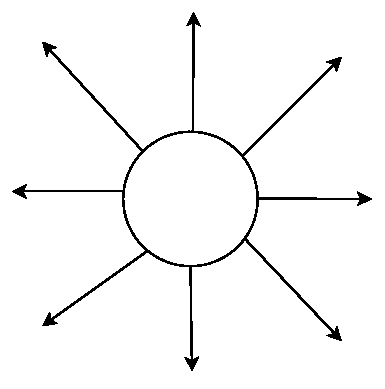
\includegraphics[scale=1]{/Users/ohyamasan/Downloads/efig.pdf}
	\end{figure}
	\item 点磁荷$m$から距離$r$の位置における磁束密度$B$を求めよ.
	\begin{align*}
		B&=\mu_{0} H=\frac{m}{4 \pi r^{2}}\,[\rm{T}]
	\end{align*}
	\item 点磁荷$m$から距離$r$の位置を通過する磁束$\Phi$を磁束密度$B$より求めよ.
	\begin{align*}
		\Phi&=BS=m\,[\rm{Wb/m}]
	\end{align*}
\end{enumerate}

\section{$xy$直交座標系において,同量異符号の点磁荷$\pm m$が距離$l$に固定された磁気双極子が存在する.このとき以下の問いに答えよ.ただし,$x$ 方向の基準ベクトルを$\boldsymbol{i}$,$y$方向の基準ベクトルを$\boldsymbol{j}$とする}
\begin{enumerate}[(a)]
	\item 点Aに存在する磁荷$-m$が点P$(x_0,y_0)$に作る磁界$\boldsymbol{H}_{1}$を求めよ.
	\begin{align*}
		\boldsymbol{H}_{1}&=\frac{1}{4\pi \mu_{0}}\frac{-m}{\left(\left(x_{0}+\frac{l}{2}\right)^{2}+y_{0}^{2}\right)^{3/2}} \left\{ \left(x_{0}+\frac{l}{2}\right)\boldsymbol{i}+y_{0}\boldsymbol{j}\right\}\,[\rm{A/m}]
	\end{align*}
	\item 点Bに存在する磁荷$+m$が点P$(x_0,y_0)$に作る磁界$\boldsymbol{H}_{2}$を求めよ.
	\begin{align*}
		\boldsymbol{H}_{2}&=\frac{1}{4\pi \mu_{0}}\frac{m}{\left(\left(x_{0}-\frac{l}{2}\right)^{2}+y_{0}^{2}\right)^{3/2}} \left\{ \left(x_{0}-\frac{l}{2}\right)\boldsymbol{i}+y_{0}\boldsymbol{j}\right\}\,[\rm{A/m}]
	\end{align*}
	\item 点Pでの磁界$\boldsymbol{H}$を求めよ.
	\begin{align*}
		\boldsymbol{H}&=\boldsymbol{H}_{1}+\boldsymbol{H}_{2}\\
		&=\frac{m}{4\pi \mu_{0}}\left[\frac{-1}{\left(\left(x_{0}+\frac{l}{2}\right)^{2}+y_{0}^{2}\right)^{3/2}} \left\{ \left(x_{0}+\frac{l}{2}\right)\boldsymbol{i}+y_{0}\boldsymbol{j}\right\}+\frac{1}{\left(\left(x_{0}-\frac{l}{2}\right)^{2}+y_{0}^{2}\right)^{3/2}} \left\{ \left(x_{0}-\frac{l}{2}\right)\boldsymbol{i}+y_{0}\boldsymbol{j}\right\}\right]\,[\rm{A/m}]
	\end{align*}
	\item 磁気双極子モーメント$\boldsymbol{M}$を求めよ.
	\begin{align*}
		\boldsymbol{M}&=m\boldsymbol{l}\\
		&=ml\boldsymbol{i}\,[\rm{Wb\cdot m}]
	\end{align*}
	\item 点Pが原点Oより十分遠方にあると仮定すると,$\sqrt{(x_{0}-l/2)^{2}+y_{0}^{2}}\simeq \sqrt{x_{0}^{2}+y_{0}^{2}}$及び$\sqrt{(x_{0}+l/2)^{2}+y_{0}^{2}} \simeq \sqrt{x_{0}^{2}+y_{0}^{2}}$と近似できる.このことを用いて(c)にて得た磁界$\boldsymbol{H}$を簡略化せよ.
	\begin{align*}
		\boldsymbol{H}&\simeq \frac{1}{4\pi \mu_{0}}\frac{ml}{\left(x_{0}^{2}+y_{0}^{2}\right)^{3/2}} \boldsymbol{i}\,[\rm{A/m}]\\
		&\left(\simeq\frac{\boldsymbol{M}}{4\pi \mu_{0}r^{3}}\,[\rm{A/m}]\right)
	\end{align*}
	\item $y$方向に一様な磁界$\boldsymbol{H}_{0}$が存在するとき,磁気双極子にはたらくトルク$T$を求めよ.
	\begin{align*}
		\boldsymbol{T}&=\boldsymbol{M}H_{0}\sin \theta \\
		&=ml\boldsymbol{i}\sin \frac{\pi}{2}\\
		&=ml\boldsymbol{i}\\
		|\boldsymbol{T}|&=ml\,[\rm{Wb\cdot m}],x軸右方向
	\end{align*}
\end{enumerate}

\section{強磁性体,常磁性体,反磁性体の3つの磁性体の性質を,比透磁率と磁化率を用いて説明せよ.}
強磁性体は磁化率が0よりかなり大きく,透磁率が1よりかなり大きい磁性体を指す.そのため,磁界と同じ方向に磁化され,その大きさも大きい.

常磁性体は磁化率が0より大きく,透磁率は1未満の磁性体を指す.そのため,磁界と同じ方向に磁化され,その大きさは大きくない.

反磁性体は磁化率が0より小さく,透磁率が1より小さい磁性体を指す.そのため,磁界と逆方向に磁化され,その大きさは小さい.

\end{document}